\chapter{Leçon 20: Medien an den Alldag}

\section{Medien an Informatioun / Médias et Informations / Media and Information}

D'Medien spillen eng grouss Roll an eisem Liewen. Wouhir kritt Dir Är Informatiounen? \textit{Les médias jouent un grand rôle dans notre vie. D'où tirez-vous vos informations ? / The media play a large role in our lives. Where do you get your information from?}

\begin{itemize}
    \item \textbf{Wéi informéiert Dir Iech?} (Comment vous informez-vous ? / How do you inform yourself?)
    \item \textbf{Wat fir Medien benotzt Dir?} (Quels médias utilisez-vous ? / What media do you use?)
    \item \textbf{Gleeft Dir de Medien?} (Croyez-vous les médias ? / Do you believe the media?)
    \item \textbf{Sinn d'Medien glafwierdeg?} (Les médias sont-ils crédibles ? / Are the media credible?)
    \item \textit{Synonymer: glafwierdeg, glafwürdeg, credibel.}
    \item \textbf{Et hänkt vun de Journalisten of. Et gi vill onofhängeg oder fräiberufflech Journalisten.} (Cela dépend des journalistes. Il y a beaucoup de journalistes indépendants ou freelances. / It depends on the journalists. There are many independent or freelance journalists.)
\end{itemize}

\subsection{Ënnerscheed tëscht "Gleewen un" an "Gleewen"}
\begin{itemize}
    \item \textbf{Ech gleewen him.} (Je le crois [lui]. / I believe him. -- \textit{On croit ce que la personne dit.})
    \item \textbf{Ech gleewen un hien.} (Je crois en lui. / I believe in him. -- \textit{On a confiance en cette personne.})
\end{itemize}

\subsection{Aarte vu Medien / Types de médias / Types of media}
\begin{itemize}
    \item \textbf{Ech benotzen den Internet op mengem Handy.} (J'utilise internet sur mon portable. / I use the internet on my mobile phone.)
    \item \textbf{Ech hu keng Zäit op menger Aarbecht fir op mäin Handy ze kucken.} (Je n'ai pas le temps, à mon travail, de regarder mon portable. / I don't have time at work to look at my phone.)
    \item \textbf{Ech lauschtere Radio an ech kucken Telee.} (J'écoute la radio et je regarde la télé. / I listen to the radio and I watch TV.)
    \item \textbf{Ech hu keng Telee.} (Je n'ai pas de télé. / I don't have a TV.)
    \item \textbf{Ech liesen Noriichten um Internet, zum Beispill "BBC", "Sky News", "L'essentiel", a "Lëtzebuerger Wort".} (Je lis les actualités sur internet, par exemple "BBC", "Sky News", "L'essentiel", et le "Lëtzebuerger Wort". / I read the news on the internet, for example "BBC", "Sky News", "L'essentiel", and "Lëtzebuerger Wort".)
    \item \textbf{Reegelméisseg lauschteren ech och Podcasten.} (Régulièrement, j'écoute aussi des podcasts. / Regularly, I also listen to podcasts.)
\end{itemize}

\subsection{Reaktiounen oppen / Réactions ouvertes / Open reactions}
\begin{itemize}
    \item \textbf{Éierlech gesot, ech kucken heiansdo den RTL Journal.} (Honnêtement / À vrai dire, je regarde de temps en temps le journal de RTL. / Honestly / To tell the truth, I sometimes watch the RTL news.)
    \item \textbf{Ech muss mech informéieren.} (Je dois m'informer. / I must inform myself.)
    \item \textbf{Heiansdo iergere ech mech... dat war op der Telee gesot!} (Parfois je me fâche... c'était dit à la télé ! / Sometimes I get angry... that was said on TV!)
    \item \textit{Notiz: Den Ierger ass d'Substantiv fir la colère / the anger.}
\end{itemize}

\subsection{Allgemeng Beispiller / Exemples généraux / General examples}
\begin{itemize}
    \item \textbf{Allgemeng liesen ech vill Bicher fir eng nei Erfarung ze maachen.} (En général, je lis beaucoup de livres pour faire une nouvelle expérience. / In general, I read many books to gain a new experience.)
    \item \textbf{Op der Tankstell: Den Diesel zu Esch kascht 1,20 Euro, maach däin Auto voll.} (À la station-service : le diesel à Esch coûte 1,20 euro, fais le plein de ta voiture. / At the petrol station: diesel in Esch costs 1.20 euros, fill up your car.)
\end{itemize}

\vspace{1cm}

\section{Verschidden Ausdréck / Expressions Diverses / Random Expressions}
Ee puer nëtzlech Wierder an Ausdréck fir den Alldag. \textit{Quelques mots et expressions utiles pour le quotidien. / Some useful words and expressions for everyday life.}

\begin{itemize}
    \item \textbf{Um Schouss} (Sur les genoux / On the lap).
    \item \textbf{Dat ass ganz locker.} (C'est très détendu, décontracté. / That is very relaxed, loose.)
    \item \textbf{Et fänkt un ze brennen a mir gesi schwaarz Wolleken.} (Ça commence à brûler et nous voyons des nuages noirs. / It starts to burn and we see black clouds.)
    \item \textbf{Eppes ass verschwonnen oder alles ass futti.} (Quelque chose a disparu ou tout est cassé. / Something has disappeared or everything is broken.)
    \item \textbf{D'Leit si leider gestuerwen.} (Les gens sont malheureusement morts. / The people unfortunately died.)
    \item \textbf{Dat eelst Kand ass 16 Joer al.} (L'enfant aîné a 16 ans. / The oldest child is 16 years old.)
    \item \textbf{Ee muss net vereinfachen an aus enger Méck en Elefant maachen.} (Il ne faut pas simplifier et faire d'une mouche un éléphant / en faire toute une montagne. / One must not simplify and make a mountain out of a molehill.)
    \item \textbf{Vereinfacht gesot...} (En d'autres termes plus simples... / Simply put...)
    \item \textbf{Woumat kann ech Iech hëllefen?} (En quoi puis-je vous aider ? / How can I help you? \textit{(With what)})
    \item \textbf{Hutt Dir an der Mëttesstonn zou?} (Êtes-vous fermé vers l'heure de midi ? / Are you closed during lunchtime?)
    \item \textbf{Muss ee bei Iech Drénkgeld ginn?} (Doit-on donner un pourboire chez vous ? / Must one give a tip here?)
\end{itemize}

\vspace{1cm}

\section{E Gespréich iwwer den Alldag / Une conversation sur le quotidien / A conversation about everyday life}
\begin{itemize}
    \item \textbf{A:} Wéini schellt däi Wecker an der Moyenne? (Quand ton réveil sonne-t-il en moyenne ? / When does your alarm clock ring on average?)
    \item \textbf{B:} Mäi Wecker schellt rëm um sechs Auer. Ech gi meeschtens direkt waakreg. Wat ass mat dir, wéini gees du waakreg? (Mon réveil sonne à nouveau à six heures. Je me réveille généralement tout de suite. Et toi, quand te réveilles-tu ? / My alarm clock rings again at six. I usually wake up right away. What about you, when do you wake up?)
    \item \textbf{A:} Ech schlofe méi laang, mee ech profitéiere vun der Mëttesrou fir ze raschten. (Je dors plus longtemps, mais je profite du repos de midi pour me reposer. / I sleep longer, but I take advantage of the midday rest to relax.)
    \item \textbf{B:} Dat ass gutt. Dann nom Feierowend hu mir genuch Zäit fir zesummen z'iesse goen. (C'est bien. Alors après la fin de la journée de travail, nous avons assez de temps pour aller manger ensemble. / That's good. Then after work is over, we have enough time to go eat together.)
\end{itemize}

\vspace{1cm}

\section{Noriichten liesen: RTL Artikel / Lire les actualités: Article RTL / Reading News: RTL Article}
Hei ass e kuerzen Artikel vun RTL (Quell:\footnote{https://www.rtl.lu/news/national/et-ass-ee-schockeiert-et-feelen-engem-dwierder-812395556}). \textit{Voici un court article de RTL. / Here is a short RTL article.}

\textbf{Vandalismus an der Schoul vu Rued-Sir: "Et ass ee schockéiert. Et feelen engem d'Wierder"} \\
(Vandalisme dans l'école de Roodt-sur-Syre : "On est choqué. Les mots nous manquent" / Vandalism in the school of Roodt-sur-Syre: "One is shocked. Words fail us")

\textbf{Iwwer 100.000 Euro Schued gouf et um Ouschterweekend. Eng Enquête leeft. D'Experte vun der Assurance waren um Mëttwochmoien am Schoulgebai sech de Schued ukucke komm.} \\
(Plus de 100 000 euros de dégâts ont eu lieu lors du week-end de Pâques. Une enquête est en cours. Les experts de l'assurance sont venus mercredi matin au bâtiment scolaire pour constater les dégâts. / There was over 100,000 euros in damage over the Easter weekend. An investigation is ongoing. The insurance experts came on Wednesday morning to the school building to look at the damage.)

\textbf{“Et freet ee sech, firwat esou eppes geschitt. Déi kriminell Energie, déi déi Leit haten. Déi Loscht, einfach nëmmen eppes ze zerstéieren”. Dëst seet de Marc Ries, Buergermeeschter vu Betzder am RTL-Interview.} \\
("On se demande pourquoi une telle chose arrive. L'énergie criminelle que ces gens avaient. Cette envie de simplement détruire quelque chose". C'est ce que dit Marc Ries, bourgmestre de Betzdorf lors de l'interview à RTL. / "One wonders why such a thing happens. The criminal energy that these people had. This desire to simply destroy something". This is what Marc Ries, mayor of Betzdorf, says in the RTL interview.)

\textbf{“Et ass e Wee vun der Verwüüstung, dat sech duerch d’ganzt Gebai zitt. Déi Leit musse relativ laang hei gewiescht sinn. Si hu geziilt ee Klassesall nom anere geholl. Insgesamt 9 Säll si komplett zerstéiert”.} \\
("C'est un chemin de dévastation qui traverse tout le bâtiment. Ces gens doivent avoir été ici relativement longtemps. Ils ont délibérément pris une salle de classe après l'autre. Au total, 9 salles sont complètement détruites". / "It is a path of devastation that runs through the entire building. These people must have been here for a relatively long time. They specifically took one classroom after another. In total, 9 rooms are completely destroyed".)

\textbf{An de leschte Woche gouf et an der Gemeng Betzder scho Probleemer mat Vandalismus. Feierläscher goufen an ëffentleche Gebaier eidel gemaach. Zwou ëffentlech Toilette goufe rezent zerstéiert.} \\
(Ces dernières semaines, il y avait déjà eu des problèmes de vandalisme dans la commune de Betzdorf. Des extincteurs ont été vidés dans des bâtiments publics. Deux toilettes publiques ont été récemment détruites. / In recent weeks, there had already been problems with vandalism in the municipality of Betzdorf. Fire extinguishers were emptied in public buildings. Two public toilets were recently destroyed.)

\textbf{De Buergermeeschter geet och dovunner aus, dass déi Persoun/déi Persoune sech am Gebai auskannt hunn. Ronderëm d’Schoul hänken nämlech 4 Kameraen um Site. Op kenger wäre Persounen drop z’erkennen. D’Brigange sinn iwwer eng Fënster oder Dier erakomm. Genee wär dat den Ament nach net festzestellen.} \\
(Le bourgmestre suppose aussi que cette personne/ces personnes connaissaient le bâtiment. En effet, 4 caméras sont installées sur le site autour de l'école. Sur aucune, il n'y aurait de personnes reconnaissables. Les voyous sont entrés par une fenêtre ou une porte. Cela ne serait pas encore possible de le déterminer exactement pour le moment. / The mayor also assumes that this person/these persons were familiar with the building. Specifically, 4 cameras are hanging around the school site. No persons would be recognizable on any of them. The thugs entered through a window or door. That could not yet be determined exactly at this moment.)

\textbf{Eemol am Schoulgebai huet d’Zerstéierung ugefaangen. De Gros vun der Verwüüstung ass um 1. Stack geschitt. Zwee Feierläscher goufen an enger Bar fonnt.} \\
(Une fois dans le bâtiment scolaire, la destruction a commencé. Le plus gros de la dévastation s'est passé au 1er étage. Deux extincteurs ont été trouvés dans un bar. / Once inside the school building, the destruction started. The bulk of the devastation happened on the 1st floor. Two fire extinguishers were found in a bar.)

\textbf{“Si hu geziilt all Computer mat héchstwarscheinlech engem Feierläscher zerstéiert. Och Laptop an Ecran. Och déi digital Tafele goufen zerstéiert. Op wäit iwwer 100.000 Euro Schued gëtt dës muttwëlleg Zerstéierung chiffréiert.”} \\
("Ils ont ciblé et détruit tous les ordinateurs, très probablement avec un extincteur. Aussi les ordinateurs portables et les écrans. Même les tableaux numériques ont été détruits. Cette destruction malveillante est chiffrée à bien plus de 100 000 euros de dégâts." / "They purposefully destroyed all computers, most likely with a fire extinguisher. Also laptops and screens. Even the digital boards were destroyed. This malicious destruction is estimated at well over 100,000 euros in damage.")

\textbf{“Ech hoffen, datt se fonnt ginn. Datt se zur Verantwortung gezu ginn. Datt se eng Konsequenz erliewen”. Dëst seet d’Marie-Claire Ruppert, 1. Schäffe vun der Gemeng Betzder.} \\
("J'espère qu'ils seront trouvés. Qu'ils seront tenus responsables. Qu'ils subiront une conséquence". C'est ce que dit Marie-Claire Ruppert, 1ère échevine de la commune de Betzdorf. / "I hope they will be found. That they will be held accountable. That they will experience a consequence". This is what Marie-Claire Ruppert, 1st alderwoman of the municipality of Betzdorf, says.)

\textbf{Si wënscht sech awer och, dass d’Elteren doheem mat de Kanner iwwer dëse Virfall schwätzen. Dass dëst thematiséiert gëtt.} \\
(Elle souhaite cependant aussi que les parents parlent à la maison de cet incident avec les enfants. Que cela soit thématisé. / However, she also wishes that parents at home talk to their children about this incident. That this is discussed.)

\textbf{D’Police Technique war op der Plaz, fir Spueren ze sécheren. Um Mëttwochmoie waren och 2 Agente vun enger Assurancëgesellschaft an der Schoul, fir de Schued ze chiffréieren. Mëttlerweil ass och d’Botzekipp am Asaz.} \\
(La police technique était sur place pour sécuriser les traces. Mercredi matin, 2 agents d'une compagnie d'assurance étaient également à l'école pour chiffrer les dégâts. Entre-temps, l'équipe de nettoyage est aussi en intervention. / The forensic police were on site to secure evidence. On Wednesday morning, 2 agents from an insurance company were also at the school to estimate the damage. Meanwhile, the cleaning team is also deployed.)

\textbf{E Méindeg soll de Schoulbetrib no 2 Woche Vakanz nees kënnen normal ufänken. Déi Responsabel vun der Gemeng hunn eng Plainte bei der Police deposéiert.} \\
(Lundi, l'école devrait pouvoir reprendre normalement après 2 semaines de vacances. Les responsables de la commune ont déposé une plainte à la police. / On Monday, school operations should be able to start normally again after 2 weeks of holidays. The municipal officials have filed a complaint with the police.)

\textbf{All Info, all Observatioun, déi ee kann tëscht Ouschtersonndeg an Ouschterméindeg gemaach hunn, ass fir den 113.} \\
(Toute info, toute observation qu'on a pu faire entre le dimanche de Pâques et le lundi de Pâques, est pour le 113. / Any info, any observation one might have made between Easter Sunday and Easter Monday is for 113.)

\vspace{1.5cm}
\color{geminiBlue}\hrule height 1.5pt \vspace{0.5em}\color{black}
\section{Vokabulär: Medien}

\begin{itemize}
    \item \textbf{en Handy} (Pl.: d'Handyen) $\rightarrow$ un téléphone portable (a mobile phone)
    \item \textbf{eng Telee} (Pl.: d'Teleeën) $\rightarrow$ une télévision (a television)
    \item \textbf{e Radio} (Pl.: d'Radioen / d'Radios) $\rightarrow$ une radio (a radio)
    \item \textbf{e Wecker} (Pl.: d'Wecker) $\rightarrow$ un réveil (an alarm clock)
\end{itemize}

\vspace{1em}

\begin{center}
    \begin{minipage}[t]{0.48\textwidth}
        \centering
        \framebox{\parbox{0.9\linewidth}{\centering
            \vspace{0.5cm}
            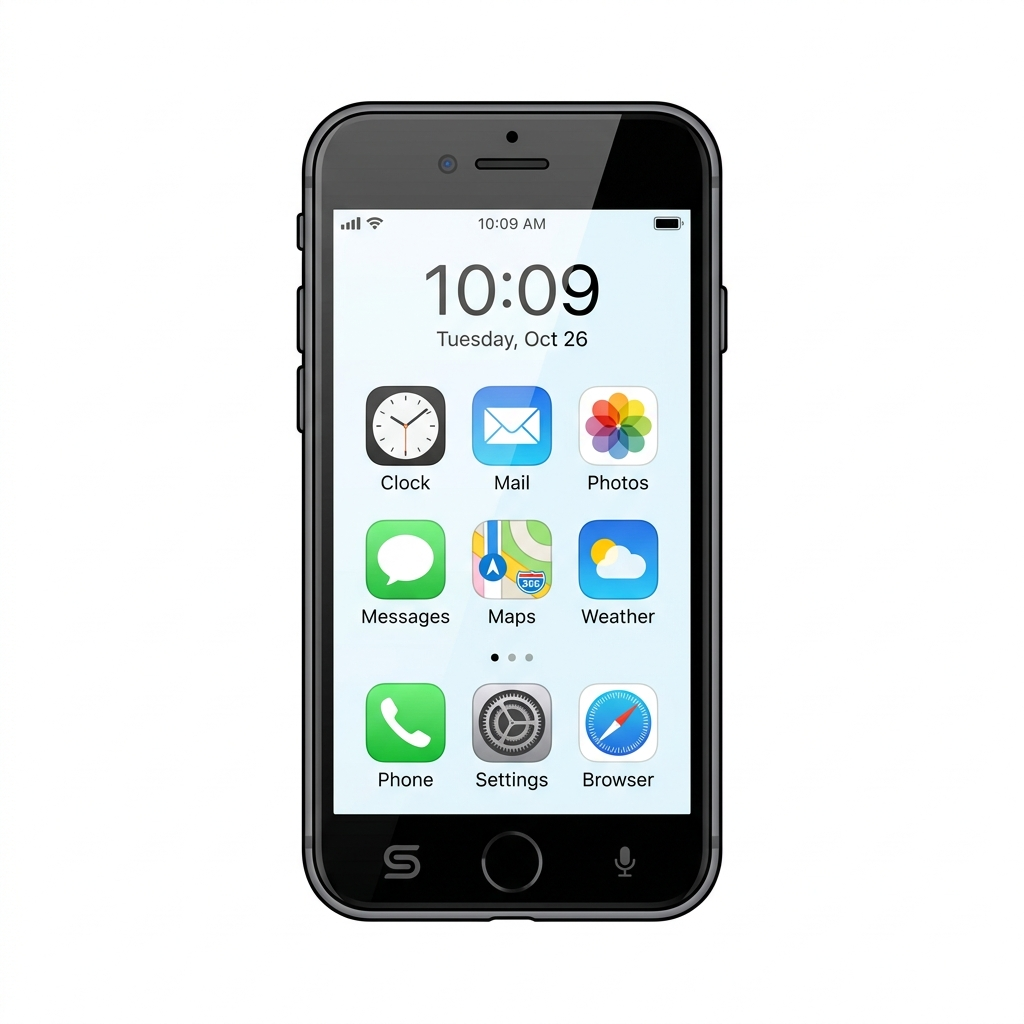
\includegraphics[width=0.9\linewidth]{vokab_300dpi/handy.png} \\
            \small\textit{En Handy (Un portable / A mobile phone)}
            \vspace{0.5cm}
        }}
    \end{minipage}
    \hfill
    \begin{minipage}[t]{0.48\textwidth}
        \centering
        \framebox{\parbox{0.9\linewidth}{\centering
            \vspace{0.5cm}
            
\includegraphics[width=0.9\linewidth]{vokab_300dpi/telee.png} \\
            \small\textit{Eng Telee (Une télévision / A television)}
            \vspace{0.5cm}
        }}
    \end{minipage}
    
    \vspace{1em}
    
    \begin{minipage}[t]{0.48\textwidth}
        \centering
        \framebox{\parbox{0.9\linewidth}{\centering
            \vspace{0.5cm}
            
\includegraphics[width=0.9\linewidth]{vokab_300dpi/radio.png} \\
            \small\textit{E Radio (Une radio / A radio)}
            \vspace{0.5cm}
        }}
    \end{minipage}
    \hfill
    \begin{minipage}[t]{0.48\textwidth}
        \centering
        \framebox{\parbox{0.9\linewidth}{\centering
            \vspace{0.5cm}
            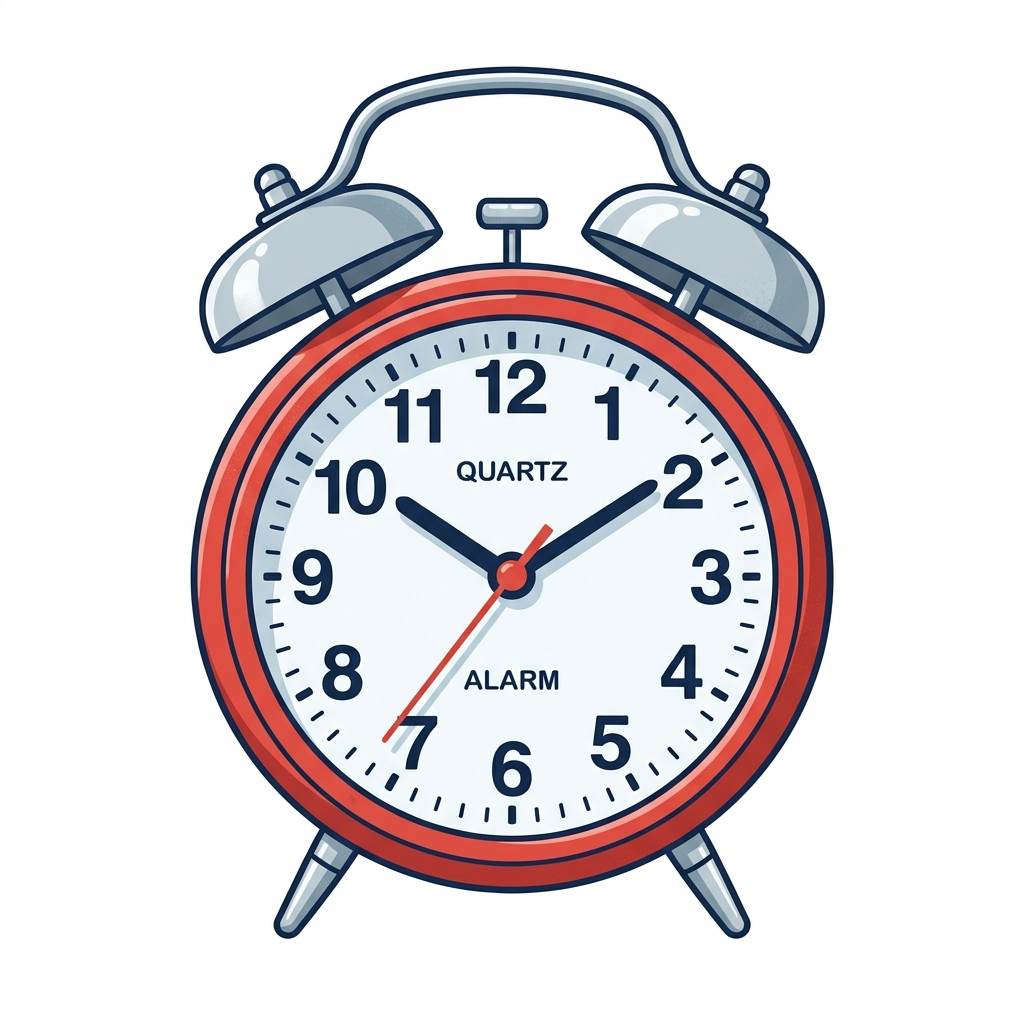
\includegraphics[width=0.9\linewidth]{vokab_300dpi/wecker.png} \\
            \small\textit{E Wecker (Un réveil / An alarm clock)}
            \vspace{0.5cm}
        }}
    \end{minipage}
\end{center}
